\documentclass[
	12pt,					        % tamanho da fonte
	openright,				    % capítulos começam em pág ímpar (insere página vazia caso preciso)
	%oneside,				      % para impressão apenas no verso
	a4paper,				      % tamanho do papel
	chapter=TITLE,			  % títulos de capítulos convertidos em letras maiúsculas
	section=TITLE,			  % títulos de seções convertidos em letras maiúsculas
	%subsection=TITLE,		% títulos de subseções convertidos em letras maiúsculas
	%subsubsection=TITLE,	% títulos de subsubseções convertidos em letras maiúsculas
	% -- opções do pacote babel --
	english,			      	% idioma adicional para hifenização
	brazil,					      % o último idioma é o principal do documento
]{abntex2}

\usepackage{udesc}

\usepackage{times} % Fonte Times New Roman
\usepackage[alf]{abntex2cite} % Citar nas normas da ABNT
\usepackage[hyphenbreaks]{breakurl} % Quebrar links
\usepackage[T1]{fontenc} % Para poder copiar as palavras com acentos
\usepackage{amssymb} % O símbolo de conjunto vazio (\emptyset)
\usepackage{amsfonts} % Os símbolos dos conjuntos numéricos
\usepackage{amsmath} % Equações de múltiplas linhas
\usepackage{indentfirst} % Indentar o primeiro parágrafo também
\usepackage{float} % Para forçar a posição das figuras
\usepackage{multirow} % Row da tabela com mais de uma linha

\hypersetup{hidelinks} % Não colorir links

% Para fazer marcações:
\usepackage{color}
\usepackage{ulem}
\newcommand\hl{\bgroup\markoverwith
  {\textcolor{yellow}{\rule[-.5ex]{2pt}{2.5ex}}}\ULon}

% Para desenhar autômatos:
\usepackage{tikz}
\usetikzlibrary{automata, positioning, arrows}
\tikzset{
    node distance=3cm,
    every state/.style={semithick},
    double distance=2pt,
    every edge/.style={
        draw,
        ->,>=stealth',
        auto,
        semithick
    },
    initial text=$ $
}

% Para escrever códigos do Coq:
\usepackage{minted}
\setminted[coq]{
    breaklines=true,
    encoding=utf8
}
\usemintedstyle{borland}
\AtBeginEnvironment{minted}{\setlength{\parskip}{0 pt}}

% Para melhorar as equações:
\usepackage{amsmath} 
\usepackage{amssymb} % para usar o símbolo de conjunto vazio

% Para determinar o número da última página na ficha catalográfica:
\usepackage{lastpage}

% Para agilizar a inserção de figuras:
\newcommand{\figura}[4]{
	\begin{figure}[H]
    \caption{#1}
    \begin{center}
      #2
    \end{center}
    \legend{Fonte: #4.}
    \label{#3}
  \end{figure}
}
\newcommand{\figuradoautor}[3]{
  \figura{#1}{#2}{#3}{Elaborada pelo autor, 2021}
}

% Tabela
\newcommand{\ttable}[4][H]{
  \begin{table}[#1]
    \begin{center}
      #3
    \end{center}
    \caption{#2}
    \if #4\else
      \label{#4}
    \fi
  \end{table}
}

% Para agilizar a inserção de quadros:
\def\arraystretch{1.3}
\newcommand{\novoquadro}[4]{
	\begin{quadro}[H]
		\footnotesize
		\caption{#1}
		\vskip 8pt
		\label{#3}
		\centering
		#2
		\vskip 15pt
		\legend{Fonte: #4.}
	\end{quadro}
}
\newcommand{\quadrodoautor}[3]{
  \novoquadro{#1}{#2}{#3}{Elaborado pelo autor, 2021}
}

% Dados da capa:
\titulo{Prova do algoritmo de Brzozowski assistida por computador}
\autor{Filipe Ramos}
\local{Joinville - SC}
\instituicao{Universidade do Estado de Santa Catarina - Udesc}
\campus{Centro de Ciências Tecnológicas - CCT}
\curso{Bacharelado em Ciência da Computação}
\data{2021}
\fulldata{xx de xxxx de 2021}

% Dados da folha de rosto:
\inforosto{Trabalho de Conclusão de Curso apresentado ao curso de Bacharelado em Ciência da Computação como requisito parcial para a obtenção do título de Bacharel em Ciência da Computação.}
\orientador{Karina Girardi Roggia}
\orientadorRotulo{Dra. }
\coorientador{Rafael Castro Gonçalves Silva}
\coorientadorRotulo{Me. }

\begin{document}

  %!TEX root = ../Principal.tex
% Capa do trabalho
\imprimircapa


% Folha de rosto
%* indica que tem ficha catalográfica
\imprimirfolhaderosto*


% Caso a Biblioteca da UDESC forneça, utilize o comando
% \begin{fichacatalografica}
%     \includepdf{fig_ficha_catalografica.pdf}
% \end{fichacatalografica}

% Geração da ficha catalográfica via LaTeX
\begin{fichacatalografica}
	\vspace*{\fill}					% Posição vertical
	\begin{center}					% Minipage Centralizado
	\begin{minipage}[c]{12.5cm}		% Largura
	
	\imprimirautor
	
	\hspace{0.5cm} \imprimirtitulo  / \imprimirautor. --
	\imprimirlocal, \imprimirdata-
	
	\hspace{0.5cm} \pageref{LastPage} p. : il. (algumas color.) ; 30 cm.\\
	
	\hspace{0.5cm} \imprimirorientadorRotulo~\imprimirorientador\\
	
	\hspace{0.5cm}
	\parbox[t]{\textwidth}{\imprimirtipotrabalho~--~\imprimirinstituicao,
	\imprimirdata.}\\
	
	\hspace{0.5cm}
		1. Tópico 01.
		2. Tópico 02.
		I. Prof. Dr. xxxxx.
		II. Universidade do Estado de Santa Catarina.
		III. Centro de Educação do Planalto Norte.
		IV. identificação xxxx\\ 			
	
	\hspace{8.75cm} CDU 02:121:005.7\\
	
	\end{minipage}
	\end{center}
\end{fichacatalografica}


% Folha de aprovação
% Exemplo de folha de aprovação antes da Banca. Após isso, incluia o pdf digitalizado com as assinaturas%
% \includepdf{folhadeaprovacao_final.pdf}
\begin{folhadeaprovacao}

	\begin{center}
		{\ABNTEXchapterfont\bfseries\imprimirautor}
		\vspace{6em}

			\ABNTEXchapterfont\bfseries\imprimirtitulo
		
	\end{center}
		\vspace{1em}
		{\justify
		Trabalho de Conclusão de Curso apresentado ao curso de Bacharelado em Ciência da Computação como requisito parcial para a obtenção do título de Bacharel em Ciência da Computação}
	
	\vspace{3em} 
	\noindent
	{\bfseries Banca examinadora:}
	\assinatura{\textbf{Dra. Karina Girardi Roggia} \\ Instituto Superior Técnico de Lisboa} 
	\assinatura{\textbf{Dr. Cristiano Damiani Vasconcellos} \\ Universidade Federal de Minas Gerais}
    \assinatura{\textbf{Dr. Roberto Silvio Ubertino Rosso Junior} \\ Loughborough University}

    \vspace*{\fill}
    \begin{center}
    	\imprimirlocal,\,\imprimirfulldata
    \end{center}
\end{folhadeaprovacao}


% Dedicatória
\begin{dedicatoria}				
Dedico este trabalho a...  
\end{dedicatoria}


% Agradecimentos
\begin{agradecimentos}
Gostaria de agradecer...

Aqui devem ser colocadas os agradecimentos às pessoas que de alguma forma contribuíram para a realização do trabalho.
\end{agradecimentos}


% Epígrafe
\begin{epigrafe}	
``frase''
\\
\par
autor
\end{epigrafe}


% Resumo em português
\begin{resumo}
 O resumo deve ressaltar o
 objetivo, o método, os resultados e as conclusões do documento. A ordem e a extensão
 destes itens dependem do tipo de resumo (informativo ou indicativo) e do
 tratamento que cada item recebe no documento original. O resumo deve ser
 precedido da referência do documento, com exceção do resumo inserido no
 próprio documento. (\ldots) As palavras-chave devem figurar logo abaixo do
 resumo, antecedidas da expressão Palavras-chave:, separadas entre si por
 ponto e finalizadas também por ponto.

 \vspace{\onelineskip}
    
 \noindent
 \textbf{Palavras-chaves}: latex, abntex e editoração de texto.
\end{resumo}


% Resumo em inglês
\begin{resumo}[Abstract]
 \begin{otherlanguage*}{english}
	Resumo em inglês
   \vspace{\onelineskip}
 
   \noindent 
   \textbf{Key-words}: latex, abntex e text editoration.
 \end{otherlanguage*}
\end{resumo}


% Lista de figuras
\pdfbookmark[0]{\listfigurename}{lof}
\listoffigures*
\cleardoublepage


% Lista de tabelas
\pdfbookmark[0]{\listtablename}{lot}
\listoftables*
\cleardoublepage


% Lista de quadros
\pdfbookmark[0]{\listofquadrosname}{loq}
\listofquadros*
\cleardoublepage
 % texto dos elementos pré-textuais

  % Lista de abreviaturas e siglas:
  \begin{siglas}
      \acro{AFD}{Autômato finito determinístico}
      \acro{SED}{Sistema a eventos discretos}
  \end{siglas}

  % Lista de símbolos:
  % \begin{simbolos}
  %	  \SingleSpacing
  %	  \item[\%] Porcentagem
  %	  \item[$D_{ab}$] Distância Euclidiana
  %	  \item[$O(n)$] Ordem de um algoritmo
  % \end{simbolos}

  % Sumário:
  \pdfbookmark[0]{\contentsname}{toc}
  \tableofcontents*
  \cleardoublepage

  \textual

  % Retira o nome do capítulo do header:
  \pagestyle{eudesc}
  \aliaspagestyle{chapter}{eudesc}

  % Texto principal do TCC:
  \chapter{Introdução}

\section{Isomorfismo de Curry-Howard}

Esta seção visa mostrar como as provas escritas em lógica intuicionista correspondem a programas da linguagem funcional. Para tanto, utilizaremos a noção de tipos das linguagens de programação a fim de relacionar as proposições intuicionistas com estes. A relação que construiremos será a seguinte. Sejam $P$ uma proposição qualquer e $P'$ qualquer tipo correspondente. Deverá existir, então, uma prova para $P$ se e somente se houver algum termo válido do tipo $P'$. Este termo será computado por um programa, razão pela qual designaremos como provas os programas cujo objetivo seja esta correspondência. A fins de simplificação, falaremos em existência de termos quando eles forem corretamente tipados; assim, poderemos poupar a palavra válido após qualquer frase de existência.

Inicialmente demonstremos que, para quaisquer proposições $P$ e $Q$ e respectivos tipos correspondentes $P'$ e $Q'$, existe uma prova para $P \star Q$ se e somente se há um termo válido do tipo $P' \ast Q'$. Aqui $\star$ é um conectivo lógico e $\ast$, o conjunto de todos os construtores para o tipo correspondente $P' \ast Q'$.

Supondo $\star = \vee$, podemos ter dois construtores para $\ast = \oplus$:

$$\oplus := \{ \textsf{left}, \textsf{right} \}$$ em que $\textsf{left} : P' \to P' \oplus Q'$ é o construtor que recebe como entrada termo do tipo $P'$ e $\textsf{right} : Q' \to P' \oplus Q'$ é o que recebe termo do tipo $Q'$. Esse isomorfismo é facilmente validado deste modo. ($\Rightarrow$) Por definição, $P \vee Q$ tem prova se (i) $P$ ou (ii) $Q$ têm prova. Assim, há (i) $p:P'$ ou (ii) $q:Q'$ e, portanto, (i) $\textsf{left} (p)$ ou (ii) $\textsf{right} (q)$. ($\Leftarrow$) Já se há $x:P' \oplus Q'$, então $x$ é gerado por um dos construtores: (i) $\textsf{left} (p)$ com algum $p:P'$ ou (ii) $\textsf{right} (q)$ com algum $q:Q'$. Dessarte, há prova para (i) $P$ ou (ii) $Q$, como queríamos demonstrar.

De maneira semelhante, para $\star = \wedge$ e $\ast = \otimes$:

$$\otimes := \{ \textsf{and} \}$$ em que $\textsf{and} : P' \to Q' \to P' \otimes Q'$ é o construtor que recebe termos dos tipos $P'$ e $Q'$ respectivamente. ($\Rightarrow$) Se há prova para $P \wedge Q$, então também há para $P$ e $Q$ -- existem, pois, $p:P'$ e $q:Q'$. Por conseguinte, $\textsf{and} (p, q)$ é termo válido do tipo $P' \otimes Q'$. ($\Leftarrow$) Por outro lado, quando há $x:P' \otimes Q'$, $x = \textsf{and} (p, q)$ para algum $p:P'$ e algum $q:Q'$. Logo, deve existir prova para $P \wedge Q$.

No caso da implicação, o tipo correspondente é o funcional; ou seja, $P \Rightarrow Q$ é passível de prova se e somente se existe função do tipo $P' \to Q'$. Para entender essa correspondência, vale visualizar a estrutura de uma função $f:P' \to Q'$:

$$f (p:P') := \textsf{\textbf{return} } q:Q'$$ Toda função se constitui de um escopo, conjunto de todas as variáveis que são usadas ou não por ela para computar um resultado. Neste contexto, as variáveis\footnote{Considerando apenas as variáveis atribuídas} -- que são termos corretamente tipados -- correspondem a provas ou hipóteses de certas proposições. O escopo engloba as variáveis globais -- que seriam os teoremas já provados e axiomas -- e os argumentos. Assim, ao inserir-se um argumento, supõe-se um novo termo no escopo da função, o que equivale à noção de implicação ou suposição lógica.

Uma regra de inferência muito empregada na prova de teoremas é a eliminação da implicação ou \textit{modus ponens}:

$$\frac{P \Rightarrow Q, P}{\therefore Q}$$ que é facilmente obtida na programação a partir da aplicação da função correspondente à prova de $P \Rightarrow Q$ sobre o termo de tipo correspondente de $Q$:

$$f:P' \to Q'$$ $$p:P'$$ $$f(p):Q'$$ conforme havíamos definido.

A negação lógica $\lnot P$ é definida a partir da implicação: $$\lnot P := P \Rightarrow \textsf{F}$$ Outrossim, o tipo correspondente pode ser $$\sim P' := P \to \textsf{F}'$$ sendo $\textsf{F}'$ um tipo vazio, sem construtores, o que significa

$$\nexists p : \textsf{F}'$$ Portanto, nunca haverá prova para a proposição correspondente, identicamente à proposição vazia.

Se quisermos adicionar, ainda, um tipo a corresponder com a proposição tautológica, bastará-nos definir um construtor sem argumentos; por exemplo, $\textsf{true}: \varnothing \to \textsf{T}'$. Claramente, $\textsf{true}()$ serve de prova para a tautologia.

Utilizamos, muitas vezes, quantificadores lógicos em nossas proposições, como:

$$Q := \forall x:X, P(x)$$ em que $P$ é uma proposição que depende do valor de $x$, sendo $X$ um tipo qualquer. Seguindo nosso raciocínio, o correspondente de $P$ deve ser um tipo dependente, da mesma maneira. Um termo de $Q'$ seria da forma

$$f(x:X) := \textsf{\textbf{return} } p : (P' (x))$$ Sendo assim, $f$ seria capaz de gerar um termo válido $p$ do tipo que dependesse de qualquer argumento. Em outras palavras, $f$ retornaria, para todo e qualquer $x:X$ de entrada, um termo do tipo dependente $P'(x)$ -- o isomorfismo faz-se evidente. Aqui reside um possível questionamento: qual é o tipo de $f$? Explicitar isso visando a um entendimento fácil não é muito trivial, mas no CIC seria feito semelhantemente a $$f:(\forall' x:X, P'(x))$$ estreitando a relação entre tal cálculo e a lógica intuicionista.

Já o quantificador existencial

$$Q := \exists x:X, P(x)$$ é demonstrado por meio de um $x:X$ qualquer e de uma prova de $P(x)$. Sejam $x_0:X$ um termo qualquer, o construtor existencial $$\textsf{exist}:(\forall' x:X, P'(x) \to \exists' x:X, P'(x)))$$ e $p:P'(x_0)$ o correspondente de prova para $P(x_0)$, o termo $\textsf{exist}(x_0)(p):(\exists' x:X, P'(x))$ corresponde a uma prova de $Q$.

Uma relação importante e que estará presente no decorrer deste trabalho é a de igualdade. Possivelmente determinamos um construtor para o tipo correspondente dela destarte:

$$\textsf{refl}(x:X) : (x =' x)$$ novamente mediante um tipo dependente. Além disso, para demonstrar diversas igualdades e outras relações, precisamos da técnica de prova por indução, que, no presente isomorfismo, corresponde à recursão de funções. De modo a simplificar a elucidação, tenhamos de exemplo o tipo dos naturais ($\mathbb{N}$). Vamos representar esses números na forma unária, já que é fácil de compreender e implementar. Para tanto, usaremos dois construtores: um vazio e outro que recebe um natural (de maneira recursiva). Aquele representará o zero ($0$) e este ($S (n:\mathbb{N})$), o sucessor de $n$. Assim, na prática da nossa representação, teremos os termos da \autoref{tab:unarios}.

\ttable{Naturais em representação unária e decimal}{
  \begin{tabular}{c c}
    \hline
    \textbf{Representação unária} & \textbf{Decimal} \\
    \hline
    $0$ & $0$ \\ 
    $S(0)$ & $1$ \\
    $S(S(0))$ & $2$ \\
    $S(S(S(0)))$ & $3$ \\
    $S(S(S(S(0))))$ & $4$ \\
    $S(S(S(S(S(0)))))$ & $5$ \\
    $\vdots$ & $\vdots$ \\
    \hline
  \end{tabular}
}{tab:unarios}

Agora, examinemos a função \begin{equation*}\begin{split}
f(p_0, p_n) :=\textsf{ }& \textsf{rec}(0) := p_0 \\
& \textsf{rec}(S (n)) := p_n (n) (\textsf{rec}(n)) \\
& \textsf{\textbf{return} }\textsf{rec}
\end{split}\end{equation*}

\noindent
em que $p_0 : P'(0)$ corresponde à hipótese de alguma proposição $P$ sobre o zero e $p_n$ é do tipo $\forall' n:\mathbb{N}, P'(n) \to P'(S(n))$. Dentro da função $f$, definimos outra função, $\textsf{rec}$, separando em casos distintos para cada construtor dos naturais. Observando os tipos acima, notamos que $p_0$ equivale à base da prova por indução e $p_n(n, h)$ para qualquer $n:\mathbb{N}$, ao passo indutivo, sendo $h$ o equivalente à hipótese de indução.

Uma prova completa da correspondência de Curry-Howard vai além \cite{rafael_tcc}. Não obstante, com o exposto, podemos captar as noções principais para o entendimento do funcionamento do assistente de provas Coq neste trabalho de conclusão de curso. Tal sistema computacional funciona como um verificador de provas ao passo que valida os programas que construímos (ou seja, provas).
  \include{capitulos/assistente}
  \chapter{Autômatos finitos}

Um autômato finito não-determinístico (AFND), ou simplesmente autômato finito (AF), é a abstração de uma máquina que decide uma linguagem regular. Para isso, ela conta com um conjunto de estados e regras de transição definida com base em um alfabeto, o conjunto de símbolos que são permitidos na entrada da máquina. Uma regra de transição indica os próximos estados da computação de uma palavra -- sequência de símbolos -- feita símbolo a símbol, da esquerda para a direita. O processo inicia-se nos estados iniciais e, quando termina em pelo menos um estado de aceitação, aceita a entrada. O nome não-determinístico serve para indicar a possibilidade de a computação ser não-determinística, no sentido de que pode ocorrer em mais de um estado simultaneamente. Por outro lado, um autômato finito determinístico (AFD) não compartilha dessa característica, havendo, portanto, apenas um estado inicial e regras de transição determinísticas: a partir de um estado e símbolo, só é possível transicionar para um único estado.

\citeonline{van2007practical} definem um AF $G$ como uma quíntupla \begin{equation}
  \label{eq:afnd_def_1}
  G = (\Sigma, S, I, \delta, F)
\end{equation} respectivamente o alfabeto, o conjunto de estados, o conjunto de estados inciais, o conjunto de regras de transição -- ou função parcial de transição -- e o conjunto de estados finais, ou de aceitação. Notadamente, essa definição vem com algumas restrições, conforme o \autoref{quadro:afnd_restricoes}. É interessante torná-las restrições intrínsecas ao tipo que definiremos em vez de utilizar condicionais, pois facilita as provas no Coq por alguns motivos: as restrições ficam implícitas e o compilador consegue verificá-las automaticamente.

\quadrodoautor{Restrições da definição de um AFND $G$}{
  \begin{tabular}{|c|c|c|}
    \hline
    & \textbf{Componente} & \textbf{Restrição} \\
    \hline
    1 & $S$ & \multirow{2}{*}{Conjunto finito} \\
    \cline{1-2}
    2 & $\Sigma$ & \\
    \cline{1-2}
    \hline
    3 & $I$ & $I \subseteq S$ \\
    \hline
    4 & $F$ & $F \subseteq S$ \\
    \hline
    5 & $\delta$ & $\delta : S \to \Sigma \to S$ \\
    \hline
  \end{tabular}
}{quadro:afnd_restricoes}

Nas seções seguintes, discutimos a representação de AFs, outras definições relevantes a este contexto e algumas aplicações.

\section{Diagrama de estados}

Para auxiliar na visualização das transições entre os estados dos autômatos, os AFs são comumente representados por diagramas de estados. Nessa representação, os estados são nós de uma estrutura semelhante a de grafos, e as transições, arestas que interligam dois nós, conforme a \autoref{fig:afd_diagrama}. Representam-se as transições cuja origem e destino são o mesmo estado por \textit{loops}: arestas que partem de um nó e terminam no mesmo.

\figuradoautor{Representação da transição de estados em um diagrama}{
    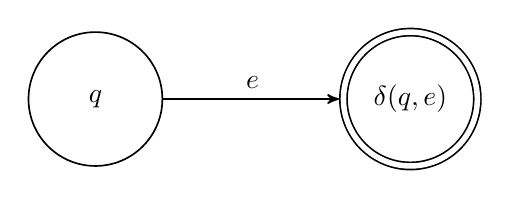
\begin{tikzpicture}[shorten >=1pt,node distance=2cm,on grid,auto] 
        \node[state,minimum size=1.7cm] (q0) {$q$}; 
        \node[state,accepting,minimum size=1.7cm] at (4,0) (q1) {$\delta(q, e)$};
        \draw
        (q0) edge node{$e$} (q1);
    \end{tikzpicture}
}{fig:afd_diagrama}

Nesta classe de diagramas, os estados inicial e final podem ser destacados de alguma forma. Para este trabalho, uma seta sem nó de origem aponta sempre para o nó do estado inicial, e uma circunferência dupla enfatiza o de um estado final, como demonstra a \autoref{fig:afd_estado_inicial}.

\figuradoautor{Representação de estados inicial (à esquerda) e final (à direita) em um diagrama}{
    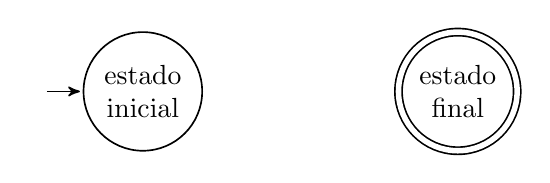
\begin{tikzpicture}[shorten >=1pt,node distance=2cm,on grid,auto] 
        \node[align=center,state,initial] (q0) {estado\\inicial};
        \node[align=center,state,accepting] at (4,0) (qf) {estado\\final};
    \end{tikzpicture}
}{fig:afd_estado_inicial}

Pode-se citar outros aspectos desta representação de autômatos: a possibilidade de adicionar rótulos aos nós, a opção de omitir os nomes dos estados nos nós quando não forem necessários e a aglutinação de transições que partem e terminam no mesmo estado em uma mesma aresta, com os símbolos separados por vírgula.

\section{Representação computacional de autômatos finitos}

Antes de iniciar qualquer prova sobre AFs no assistente de provas, devemos definir o que são esses autômatos na linguagem específica do sistema. Para tanto, precisamos utilizar estruturas de dados convencionais, pois estamos tratando de um assistente computacional. Novamente, facilita os trabalhos sequentes as restrições dos AFs representados pelas nossas estruturas de dados serem inerentes a elas.

Façamos uma singela modificação na definição da \autoref{eq:afnd_def_1}. Fixemos $$S = S' \cup I \cup F \cup \{ s \mid \exists a s', (s, a, s') \in \delta \vee (s', a, s) \in \delta \}$$ sendo o nosso conjunto de estados definido agora pela união dos estados iniciais ($I$), finais ($F$), definidos pelas transições e outros possivelmente desconexos ($S'$). Além disso, passemos a definir o alfabeto como $$\Sigma = \Sigma' \cup \{ a \mid \exists s s', (s, a, s') \in \delta \}$$ de forma semelhante, a união dos símbolos contidos em transições e dos não utilizados ($\Sigma'$). Apesar de ser uma maneira aparentemente mais complexa para o nosso entendimento do que é um AF, essa nova forma substitui as restrições condicionais de forma conveniente. Desse modo, um AF $G$ não será mais rotulado pela quíntupla da \autoref{eq:afnd_def_1}, mas por cinco novos conjuntos de componentes: \begin{itemize}
  \item conjunto finito de estados ($S'$);
  \item conjunto finito de estados iniciais ($I$);
  \item conjunto finito de estados finais ($F$);
  \item conjunto finito de símbolos ($\Sigma'$);
  \item conjutno finito de transições ($\delta$).
\end{itemize} Essa nova representação define o alfabeto ($\Sigma$) e conjunto de estados ($S$) de forma implícita, nos restando apenas agora as restrições 1 e 2 do \autoref{quadro:afnd_restricoes}.

Agora nos resta representar os conjuntos finitos supracitados como estruturas de dados computacionais. Uma abordagem comum é o uso de \textit{sets}, uma espécie de lista ordenada sem repetição \cite{blot2016sets}. A vantagem dessa estrutura é a extensionalidade: dois conjuntos são iguais se e somente se suas representações são iguais. Todavia, ela necessita de comparadores, e os algoritmos de ordenamento interferem no desempenho da computação, entre outros. No presente estudo, a ausência da propriedade extensional não obsta as provas sobre AFs uma vez que podemos substituir a relação de igualdade de conjuntos por uma nova relação de equivalência. Assim, se representarmos os conjuntos por listas simples, duas listas $L1$ e $L2$ serão ditas equivalentes se $$\forall x, x \in L1 \leftrightarrow x \in L2$$ permitindo inclusive elementos fora da ordem ou repetidos nas estruturas.

\figuradoautor{Estrutura de dados para AFs}{
}{fig:afnd_coq}

\begin{minted}{coq}
Inductive nfa_comp {A B} :=
| state (q:A)
| symbol (a:B)
| start (q:A)
| accept (q:A)
| trans (q:A) (a:B) (q':A).

Definition nfa_comp_list A B := list (@nfa_comp A B).
\end{minted}

Baseado nisso, a estrutura usada por este trabalho, já na linguagem do assistente de provas Coq, é a que segue na \autoref{fig:afnd_coq}. É importante notarmos uma nova restrição decorrente da teoria dos tipos -- implementada pelo Coq. Antes falávamos em elementos quaisquer, diferenciando-os apenas pelos conjuntos aos quais pertenciam. Ao utilizarmos tipos, no entanto, condicionamos os elementos -- agora termos -- a eles. Os termos podem ser, por exemplo, números naturais, strings ou de qualquer tipo que definirmos. Nem todos os tipos, entretanto, nos garantem uma propriedade essencial para a computação dos algoritmos sobre os AFs representados: a decidibilidade da igualdade. Um tipo $A$ tem igualdade decidível se existe algum decisor $f$ tal que $$\forall x y, f(x, y) \leftrightarrow x = y$$ Dessarte, junto aos componentes, nossa representação abarcará a restrição de existência desses decisores para os tipos \texttt{A} e \texttt{B} da \autoref{fig:afnd_coq}.

\section{Função de transição}

Uma das funções mais importantes relativas aos AFs é a de transição. A função de transição $\delta$ de um autômato $G$ é tal que $$\forall s a s', s' \in \delta(s, a) \leftrightarrow \texttt{trans}\text{ }s\text{ }a\text{ }s' \in G$$ Ela pode ser estendida para que funcione computando uma dada sequência de símbolos (lista) $w$ a partir de um dado conjunto de estados $Q$ desta maneira $$\delta(Q, \epsilon) = Q$$ $$\delta(Q, a) = \{ s \mid \exists s' a, \texttt{trans}\text{ }s'\text{ }a\text{ }s \in G \wedge s' \in Q \}$$ $$\delta(Q, aw) = \delta(\delta(Q, a), w)$$ em que $\epsilon$ é a palavra vazia e $a \in \Sigma$ é um símbolo do alfabeto do autômato. Desenvolvemos tal função facilmente no Coq, de forma segmentada. Definimos, por exemplo, uma função que recebe um estado e símbolo e, por meio de sucessivas iterações na lista que o representa, constrói uma lista de estados que são transicionados a partir daqueles; depois escrevemos uma função estendida que se utiliza dessa última para generalizar as entradas para listas de estados e símbolos. Essas funções também recebem os decisores de igualdade do AF, que suprimiremos no decorrer do presente trabalho. 

A função de transição é responsável pela computação da entrada que o autômato recebe. Temos a possibilidade de formalizar a linguagem do AF $G$ como o conjunto $$L(G) = \{ w \mid \exists s, s \in F \wedge s \in \delta(I, w) \}$$ Logo, para verificar se uma palavra é aceita pelo AF, basta-nos rodar a função de transição sobre os estados iniciais e essa dada palavra e verificar se um dos termos resultantes é estado pertencente ao conjunto de estados finais.

Outra definição importante relacionada à de transições tange aos caminhos. Essa é uma definição indutiva de dois construtores: \begin{itemize}
  \item para todo possível estado\footnote{Termo do tipo dos estados do autômato} $s$, existe um caminho de $s$ a $s$ por $\epsilon$;
  \item para todos os estados $s_1$, $s_2$, símbolo $a$ e palavra $w$, se existe uma transição $\texttt{trans}\text{ }s_2\text{ }a\text{ }s_3 \in G$ e um caminho de $s_1$ a $s_2$ por $w$, então existe um caminho de $s_1$ a $s_3$ por $wa$.
\end{itemize} A noção de caminho é relevante para tratar de buscas\footnote{Como a busca em profundidade}.

\section{Alcançabilidade dos estados}

\section{Reversão}

\section{Autômatos finitos determinísticos}

Os autômatos finitos determinísticos (AFDs) carregam duas restrições a mais: (1) possuem apenas um estado inicial e (2) as transições são determinísticas, ou seja, não existe uma transição partindo de um mesmo estado e mediante um mesmo símbolo para um estado destino diferente. Consideremos permitida a existência de AFDs sem estado inicial a fim de simplificar o presente estudo. Isso não acarretará inconsistência, uma vez que a representação de um AFD sem estado inicial é equivalente à de um AFD com um estado inicial sem transições a partir dele -- a linguagem e as propriedades de interesse do trabalho se mantêm isomórficas. Para representar os AFDs no Coq, utilizemos a mesma estrutura de dados e um tipo proposição indutivamente definido. Basicamente, esse tipo receberá construtores para cada construtor de AF, com diferenças para os construtores de estado inicial e transição. Nesses casos, adicionamos hipóteses para garantir as restrições.

Um modo de garantir a restrição (1) é criando dois construtores. O primeiro receberá um AF $G_1$ qualquer, uma prova de que ele é determinístico, uma prova de que ele não possui estados inicias e um estado inicial $q_0$. Dessa forma podemos afirmar que o o autômato $\texttt{start}\text{ }q0\texttt{::}G_1$ é determinístico. O outro construtor receberá um AF $G_2$ qualquer, uma prova de que ele é determinístico, um estado inicial $q_1$ e uma prova de que já existe um estado inicial igual a $q_1$. Outrossim, o autômato $\texttt{start}\text{ }q_1\texttt{::}G_2$ também é determinístico.

Semelhantemente, em relação à restrição (2), podemos utilizar a mesma tática. Primeiro garantimos que não existe uma transição $\texttt{trans}\text{ }q\text{ }a\text{ }s$ para todo e qualquer $s$ no AFD $G_1$ e obtemos um AFD $\texttt{trans}\text{ }q\text{ }a\text{ }q'\texttt{::}G_1$. Depois definimos que existe $\texttt{trans}\text{ }r\text{ }b\text{ }r'$ no AFD $G_2$ para termos um AFD $\texttt{trans}\text{ }r\text{ }b\text{ }r'\texttt{::}G_2$.

\section{Determinização}

\section{Aplicações}
  \chapter{Minimização de autômatos finitos determinísticos}

\section{Algoritmo de Brzozowski}
  \include{capitulos/relacionados}
  \chapter{Prova do algoritmo de Brzozowski}

\section{Provas sobre reversão}

\section{Prova do algoritmo de determinização}
  \include{capitulos/conclusao}

  % Finaliza o bookmark do PDF:
  \bookmarksetup{startatroot}

  \postextual

  % Referências bibliográficas:
  \bibliography{referencias}

  % Glossário:
  %
  % Consulte o manual da classe abntex2 para orientações sobre o glossário.
  %
  %\glossary

  % Apêndices:
  %\begin{apendicesenv}
  %	\include{Partes/apeA}
  %\end{apendicesenv}

  % Anexos:
  %\begin{anexosenv}
  %	\include{Partes/aneA}
  %\end{anexosenv}

\end{document}